%

\begin{abstract}
%

%


Off-Policy Evaluation (OPE) in contextual bandits is crucial for assessing new policies using existing data without costly experimentation. However, current OPE methods, such as Inverse Probability Weighting (IPW) and Doubly Robust (DR) estimators, suffer from high variance, particularly in cases of low overlap between target and behavior policies or large action and context spaces. In this paper, we introduce a new OPE estimator for contextual bandits, the Marginal Ratio (MR) estimator, which focuses on the shift in the marginal distribution of outcomes $Y$ instead of the policies themselves. Through rigorous theoretical analysis, we demonstrate the benefits of the MR estimator compared to conventional methods like IPW and DR in terms of variance reduction. Additionally, we establish a connection between the MR estimator and the state-of-the-art Marginalized Inverse Propensity Score (MIPS) estimator, proving that MR achieves lower variance among a generalized family of MIPS estimators. We further illustrate the utility of the MR estimator in causal inference settings, where it exhibits enhanced performance in estimating Average Treatment Effects (ATE). Our experiments on synthetic and real-world datasets corroborate our theoretical findings and highlight the practical advantages of the MR estimator in OPE for contextual bandits. 
\end{abstract}
%
%
\section{Introduction}
\label{sec:introduction}
The business processes of organizations are experiencing ever-increasing complexity due to the large amount of data, high number of users, and high-tech devices involved \cite{martin2021pmopportunitieschallenges, beerepoot2023biggestbpmproblems}. This complexity may cause business processes to deviate from normal control flow due to unforeseen and disruptive anomalies \cite{adams2023proceddsriftdetection}. These control-flow anomalies manifest as unknown, skipped, and wrongly-ordered activities in the traces of event logs monitored from the execution of business processes \cite{ko2023adsystematicreview}. For the sake of clarity, let us consider an illustrative example of such anomalies. Figure \ref{FP_ANOMALIES} shows a so-called event log footprint, which captures the control flow relations of four activities of a hypothetical event log. In particular, this footprint captures the control-flow relations between activities \texttt{a}, \texttt{b}, \texttt{c} and \texttt{d}. These are the causal ($\rightarrow$) relation, concurrent ($\parallel$) relation, and other ($\#$) relations such as exclusivity or non-local dependency \cite{aalst2022pmhandbook}. In addition, on the right are six traces, of which five exhibit skipped, wrongly-ordered and unknown control-flow anomalies. For example, $\langle$\texttt{a b d}$\rangle$ has a skipped activity, which is \texttt{c}. Because of this skipped activity, the control-flow relation \texttt{b}$\,\#\,$\texttt{d} is violated, since \texttt{d} directly follows \texttt{b} in the anomalous trace.
\begin{figure}[!t]
\centering
\includegraphics[width=0.9\columnwidth]{images/FP_ANOMALIES.png}
\caption{An example event log footprint with six traces, of which five exhibit control-flow anomalies.}
\label{FP_ANOMALIES}
\end{figure}

\subsection{Control-flow anomaly detection}
Control-flow anomaly detection techniques aim to characterize the normal control flow from event logs and verify whether these deviations occur in new event logs \cite{ko2023adsystematicreview}. To develop control-flow anomaly detection techniques, \revision{process mining} has seen widespread adoption owing to process discovery and \revision{conformance checking}. On the one hand, process discovery is a set of algorithms that encode control-flow relations as a set of model elements and constraints according to a given modeling formalism \cite{aalst2022pmhandbook}; hereafter, we refer to the Petri net, a widespread modeling formalism. On the other hand, \revision{conformance checking} is an explainable set of algorithms that allows linking any deviations with the reference Petri net and providing the fitness measure, namely a measure of how much the Petri net fits the new event log \cite{aalst2022pmhandbook}. Many control-flow anomaly detection techniques based on \revision{conformance checking} (hereafter, \revision{conformance checking}-based techniques) use the fitness measure to determine whether an event log is anomalous \cite{bezerra2009pmad, bezerra2013adlogspais, myers2018icsadpm, pecchia2020applicationfailuresanalysispm}. 

The scientific literature also includes many \revision{conformance checking}-independent techniques for control-flow anomaly detection that combine specific types of trace encodings with machine/deep learning \cite{ko2023adsystematicreview, tavares2023pmtraceencoding}. Whereas these techniques are very effective, their explainability is challenging due to both the type of trace encoding employed and the machine/deep learning model used \cite{rawal2022trustworthyaiadvances,li2023explainablead}. Hence, in the following, we focus on the shortcomings of \revision{conformance checking}-based techniques to investigate whether it is possible to support the development of competitive control-flow anomaly detection techniques while maintaining the explainable nature of \revision{conformance checking}.
\begin{figure}[!t]
\centering
\includegraphics[width=\columnwidth]{images/HIGH_LEVEL_VIEW.png}
\caption{A high-level view of the proposed framework for combining \revision{process mining}-based feature extraction with dimensionality reduction for control-flow anomaly detection.}
\label{HIGH_LEVEL_VIEW}
\end{figure}

\subsection{Shortcomings of \revision{conformance checking}-based techniques}
Unfortunately, the detection effectiveness of \revision{conformance checking}-based techniques is affected by noisy data and low-quality Petri nets, which may be due to human errors in the modeling process or representational bias of process discovery algorithms \cite{bezerra2013adlogspais, pecchia2020applicationfailuresanalysispm, aalst2016pm}. Specifically, on the one hand, noisy data may introduce infrequent and deceptive control-flow relations that may result in inconsistent fitness measures, whereas, on the other hand, checking event logs against a low-quality Petri net could lead to an unreliable distribution of fitness measures. Nonetheless, such Petri nets can still be used as references to obtain insightful information for \revision{process mining}-based feature extraction, supporting the development of competitive and explainable \revision{conformance checking}-based techniques for control-flow anomaly detection despite the problems above. For example, a few works outline that token-based \revision{conformance checking} can be used for \revision{process mining}-based feature extraction to build tabular data and develop effective \revision{conformance checking}-based techniques for control-flow anomaly detection \cite{singh2022lapmsh, debenedictis2023dtadiiot}. However, to the best of our knowledge, the scientific literature lacks a structured proposal for \revision{process mining}-based feature extraction using the state-of-the-art \revision{conformance checking} variant, namely alignment-based \revision{conformance checking}.

\subsection{Contributions}
We propose a novel \revision{process mining}-based feature extraction approach with alignment-based \revision{conformance checking}. This variant aligns the deviating control flow with a reference Petri net; the resulting alignment can be inspected to extract additional statistics such as the number of times a given activity caused mismatches \cite{aalst2022pmhandbook}. We integrate this approach into a flexible and explainable framework for developing techniques for control-flow anomaly detection. The framework combines \revision{process mining}-based feature extraction and dimensionality reduction to handle high-dimensional feature sets, achieve detection effectiveness, and support explainability. Notably, in addition to our proposed \revision{process mining}-based feature extraction approach, the framework allows employing other approaches, enabling a fair comparison of multiple \revision{conformance checking}-based and \revision{conformance checking}-independent techniques for control-flow anomaly detection. Figure \ref{HIGH_LEVEL_VIEW} shows a high-level view of the framework. Business processes are monitored, and event logs obtained from the database of information systems. Subsequently, \revision{process mining}-based feature extraction is applied to these event logs and tabular data input to dimensionality reduction to identify control-flow anomalies. We apply several \revision{conformance checking}-based and \revision{conformance checking}-independent framework techniques to publicly available datasets, simulated data of a case study from railways, and real-world data of a case study from healthcare. We show that the framework techniques implementing our approach outperform the baseline \revision{conformance checking}-based techniques while maintaining the explainable nature of \revision{conformance checking}.

In summary, the contributions of this paper are as follows.
\begin{itemize}
    \item{
        A novel \revision{process mining}-based feature extraction approach to support the development of competitive and explainable \revision{conformance checking}-based techniques for control-flow anomaly detection.
    }
    \item{
        A flexible and explainable framework for developing techniques for control-flow anomaly detection using \revision{process mining}-based feature extraction and dimensionality reduction.
    }
    \item{
        Application to synthetic and real-world datasets of several \revision{conformance checking}-based and \revision{conformance checking}-independent framework techniques, evaluating their detection effectiveness and explainability.
    }
\end{itemize}

The rest of the paper is organized as follows.
\begin{itemize}
    \item Section \ref{sec:related_work} reviews the existing techniques for control-flow anomaly detection, categorizing them into \revision{conformance checking}-based and \revision{conformance checking}-independent techniques.
    \item Section \ref{sec:abccfe} provides the preliminaries of \revision{process mining} to establish the notation used throughout the paper, and delves into the details of the proposed \revision{process mining}-based feature extraction approach with alignment-based \revision{conformance checking}.
    \item Section \ref{sec:framework} describes the framework for developing \revision{conformance checking}-based and \revision{conformance checking}-independent techniques for control-flow anomaly detection that combine \revision{process mining}-based feature extraction and dimensionality reduction.
    \item Section \ref{sec:evaluation} presents the experiments conducted with multiple framework and baseline techniques using data from publicly available datasets and case studies.
    \item Section \ref{sec:conclusions} draws the conclusions and presents future work.
\end{itemize}

\section{Background}
\subsection{Setup and Notation} \label{sec:setup_notation}
We consider the standard contextual bandit setting. Let $X\in\Xspace$ be a context vector (e.g., user features), $A\in \Aspace$ denote an action (e.g., recommended website to the user), and $Y\in \Yspace$ denote a scalar reward or outcome (e.g., whether the user clicks on the website). The outcome and context are sampled from unknown probability distributions $p(y\mid x, a)$ and $p(x)$ respectively. Let $\D\coloneqq \{(x_i, a_i, y_i)\}_{i=1}^n$ be a historically logged dataset with $n$ observations, generated by a (possibly unknown) \emph{behaviour policy} $\beh(a\mid x)$.
Specifically, $\D$ consists of i.i.d. samples from the joint density under\textit{ behaviour policy},
\begin{align}
    \pbeh(x, a, y) \coloneqq p(y\mid x, a)\, \textcolor{blue}{\beh(a\mid x)}\,p(x). \label{eq:behav-joint-factorisation}
\end{align}
We denote the joint density of $(X, A, Y)$ under the \textit{target policy} as
\begin{align}
    \ptar(x, a, y) \coloneqq p(y\mid x, a)\, \textcolor{red}{\tar(a\mid x)}\,p(x). \label{eq:tar-joint-factorisation}
\end{align}

Moreover, we use $\pbeh(y)$ to denote the marginal density of $Y$ under the behaviour policy, 
\begin{align*}
    \pbeh(y) &= \int_{\Aspace \times \Xspace} \pbeh(x, a, y)\, \mathrm{d}a \, \mathrm{d}x,
\end{align*}
and likewise for the target policy $\tar$. Similarly, we use $\Ebeh$ and $\Etar$ to denote the expectations under the joint densities $\pbeh(x, a, y)$ and $\ptar(x, a, y)$ respectively.


\myparagraph{Off-policy evaluation (OPE)}
The main objective of OPE is to estimate the expectation of the outcome $Y$ under a given target policy $\tar$, i.e., $\Etar [Y]$, using only the logged data $\D$.
%
%
%


%
%
%
%
%
%
%
%
%
%
%
%

%
%
%
%
%

Throughout this work, we assume that the support of the target policy $\tar$ is included in the support of the behaviour policy $\beh$. This is to ensure that importance sampling yields unbiased off-policy estimators, and is satisfied for exploratory behaviour policies such as the $\epsilon$-greedy policies. 
\begin{assumption}[Support]
    For any $x \in \Xspace, a \in \Aspace$,  $\tar(a\mid x) >0 \implies \beh(a\mid x) >0$. 
\end{assumption}
%
 

\subsection{Existing off-policy evaluation methodologies}
Next, we will present some of the most commonly used OPE estimators before outlining the limitations of these methodologies. This motivates our proposal of an alternative OPE estimator. 

The value of the target policy can be expressed as the expectation of outcome $Y$ under the target data distribution $\ptar(x, a, y)$.
%
%
%
%
However in most cases, we do not have access to samples from this target distribution and hence we have to resort to importance sampling methods.
\paragraph{Inverse Probability Weighting (IPW) estimator}
One way to compute the target policy value, $\Etar[Y]$, when only given data generated from $\pbeh(x, a, y)$ is to rewrite the policy value as follows:
%

\begin{small}
\begin{align*}
    \Etarred[Y] =
    \int y \, \ptar(x, a, y) \,\mathrm{d}y \, \mathrm{d}a\, \mathrm{d}x   =
    \int y \, \underbrace{\frac{\ptar(x, a, y)}{\pbeh(x, a, y)}}_{\rho(a,x)}\, \pbeh(x, a, y) \,\mathrm{d}y \, \mathrm{d}a\, \mathrm{d}x =
    %
    \Ebehblue\left[Y\,\rho(A, X)\right],
\end{align*}
\end{small} 
where 
$
\rho(a, x) \coloneqq \frac{\ptar(x, a, y)}{\pbeh(x, a, y)} = \frac{\tar(a|x)}{\beh(a|x)}
$, given the factorizations in Eqns. \eqref{eq:behav-joint-factorisation} and \eqref{eq:tar-joint-factorisation}.
This leads to the commonly used \emph{Inverse Probability Weighting (IPW)} \citep{horvitz1952generalization} estimator:
\[
\thetaipw \coloneqq \frac{1}{n}\sum_{i=1}^n \rho(a_i, x_i)\,y_i.
\]
When the behaviour policy is known, IPW is an unbiased and consistent estimator. However, it can suffer from high variance, especially as the overlap between the behaviour and target policies decreases. 

\myparagraph{Doubly Robust (DR) estimator} 
To alleviate the high variance of IPW, \cite{dudik2014doubly} proposed a \emph{Doubly Robust (DR)} estimator for OPE. 
DR uses an estimate of the conditional mean $\hat{\mu}(a, x) \approx\E[Y\mid X=x, A=a]$ (\emph{outcome model}), as a control variate to decrease the variance of IPW. It is also doubly robust in that it yields accurate value estimates if either the importance weights $\rho(a, x)$ or the outcome model $\hat{\mu}(a, x)$ is well estimated \citep{dudik2014doubly, jiang2016doubly}. 
The DR estimator for $\Etar[Y]$ can be written as follows:
\[
\thetadr = \frac{1}{n} \sum_{i=1}^n \rho(a_i, x_i)\,(y_i - \hat{\mu}(a_i, x_i)) + \hat{\eta}(\tar),
%
\]
where
$
\hat{\eta}(\tar) = \frac{1}{n} \sum_{i=1}^n \sum_{a'\in \Aspace} \hat{\mu}(a', x_i) \tar(a'\mid x_i) \approx \E_{\tar}[\hat{\mu}(A, X)]$. Here, $\hat{\eta}(\tar)$ is referred to as the Direct Method (DM) as it uses $\hat{\mu}(a, x)$ directly to estimate target policy value. 

\subsection{Limitation of existing methodologies} 
To estimate the value of the target policy $\tar$, the existing methodologies consider the shift in the joint distribution of $(X, A, Y)$  as a result of the policy shift (by weighting samples by policy ratios). As we show in Section \ref{subsec:comparison}, considering the joint shift can lead to inefficient policy evaluation and high variance especially as the policy shift increases \citep{li2018addressing}.
Since our goal is to estimate $\Etar[Y]$, we will show in the next section that considering only the shift in the marginal distribution of the outcomes $Y$ from $\pbeh(Y)$ to $\ptar(Y)$, leads to a more efficient OPE methodology compared to existing approaches.

To better comprehend why only considering the shift in the marginal distribution is advantageous, let us examine an extreme example where we assume that $Y \indep A \mid X$, i.e., the outcome $Y$ for a user $X$ is independent of the action $A$ taken. In this specific instance, $\Etar[Y] = \Ebeh[Y] \approx 1/n\sum_{i=1}^n y_i,$ indicating that an unweighted empirical mean serves as a suitable unbiased estimator of $\Etar[Y]$. However, IPW and DR estimators use policy ratios $\rho(a, x)  = \frac{\tar(a \mid x)}{\beh(a \mid x)}$ as importance weights. In case of large policy shifts, these ratios may vary significantly, leading to high variance in IPW and DR.

In this particular example, the shift in policies is inconsequential as it does not impact the distribution of outcomes $Y$. Hence, IPW and DR estimators introduce additional variance due to the policy ratios when they are not actually required. This limitation is not exclusive to this special case; in general, methodologies like IPW and DR exhibit high variance when there is low overlap between target and behavior policies \citep{li2018addressing} even if the resulting shift in marginals of the outcome $Y$ is not significant.
%

Therefore, we propose the \emph{Marginal Ratio (MR)} OPE estimator for contextual bandits in the subsequent section, which circumvents these issues by focusing on the shift in the marginal distribution of the outcomes $Y$. Additionally, we provide extensive theoretical insights on the comparison of MR to existing state-of-the-art methods, such as IPW and DR.

%
%

%

%

%






%
%
%
%

\section{Marginal Ratio (MR) estimator}
 
%
%
Our method's key insight involves weighting outcomes by the marginal density ratio of outcome $Y$:
\begin{align*}
\Etarred[Y] &= \int_{\Yspace} y \, \ptar(y)\, \mathrm{d}y = \int_\Yspace y\, \frac{\ptar(y)}{\pbeh(y)} \, \pbeh(y) \, \mathrm{d}y = \Ebehblue\left[Y\, w(Y) \right],
\end{align*}
where 
$
w(y) \coloneqq \frac{\ptar(y)}{\pbeh(y)}.
$
This leads to the Marginal Ratio OPE estimator:
\begin{align*}
    \thetamr \coloneqq \frac{1}{n}\sum_{i=1}^n w(y_i) \, y_i.
\end{align*}

In Section \ref{subsec:comparison} we prove that by only considering the shift in the marginal distribution of outcomes, the MR estimator achieves a lower variance than the standard OPE methods. In fact, this estimator does not depend on the shift between target and behaviour policies directly. Instead, it depends on the shift between the marginals $\pbeh(y)$ and $\ptar(y)$.
%
%
%
%
%

\myparagraph{Estimation of $w(y)$} When the weights $w(y)$ are known exactly, the MR estimator is unbiased and consistent. However, in practice the weights $w(y)$ are often not known and must be estimated using the logged data $\D$. Here, we outline an efficient way to estimate $w(y)$ by first representing it as a conditional expectation, which can subsequently be expressed as the solution to a regression problem.
%
%
%
%
%
%
%
\begin{lemma}\label{lemma:weights-est}
Let $w(y)=\frac{\ptar(y)}{\pbeh(y)}$ and $\rho(a, x) = \frac{\tar(a\mid x)}{\beh(a\mid x)}$, then $w(y) = \Ebeh\left[ \rho(A, X) \mid \,Y=y \right]$, and,
%
%
%
%
\begin{align}
 w = \arg\min_{f} \, \Ebeh \left[(\rho(A, X)-f(Y))^2\right]. \label{eq:weights-obj-main}
\end{align}
\end{lemma}
%
Lemma \ref{lemma:weights-est} allows us to approximate $w(y)$ using a parametric family $\{f_\phi: \mathbb{R}\rightarrow \mathbb{R} \mid \phi \in \Phi\}$ (e.g.\ neural networks) and defining $\hat{w}(y)\coloneqq f_{\phi^*}(y)$, where $\phi^*$ solves the regression problem in Eq. \eqref{eq:weights-obj-main}. 

%
%
%

%
%
%
%
%
%
%
%
%
%

%
%
%

Note that MR can also be estimated alternatively by directly estimating $h(y) \coloneqq w(y)\,y$ 
%
using a similar regression technique as above and computing $\thetamr = 1/n \sum_{i=1}^n h(y_i)$. We include additional details along with empirical comparisons in Appendix \ref{sec:alt-estimation-method}. 
%

\begin{comment}
\subsubsection{Alternative estimation method}\label{sec:alt-estimation-method}
When estimating the MR estimator, we can alternatively estimate $h(y) \coloneqq y\,w(y)$ using 
\begin{align*}
    h = \arg\min_{f} \, \Ebeh \Bigg(Y\,\frac{\tar(A|X)}{\beh (A|X)}-f(Y)\Bigg)^2.
\end{align*}
Subsequently, the MR estimator can be written as:
\[
\thetamr = \frac{1}{n}\sum_{i=1}^n h(y_i).
\]
\paragraph{Remark}
These methods outline two different methodologies of estimating MR. In general, it is difficult to say which of the two methods will perform better. Intuitively speaking, in cases where the behaviour of the quantity $Y\,\frac{\tar(A|X)}{\beh (A|X)}$ with varying $Y$ is `smoother' than that of $\frac{\tar(A|X)}{\beh (A|X)}$, the alternative method is expected to perform better. Our empirical results in Appendix \ref{app:experiments} shows that the relative performance of the two methods varies for different data generating mechanisms.

%

\rob{We could alternatively write $\Etar[Y] = \Ebeh[\Ebeh[Y \, \frac{\pi^\ast(A|X)}{\beh(A|X)} \mid Y]]$, regress $h_\theta(y) \approx \Ebeh[Y \, \frac{\pi^\ast(A|X)}{\beh(A|X)} \mid Y = y]$, and approximate $\Etar[Y] \approx \frac{1}{n} \sum_{i=1}^n h_\theta(Y_i)$. Is there a reason not to prefer this approach?}

\arnaud{indeed Rob, actually i conjecture that this should be better - think of a case where the policy ratio is high in regions where the outcome is null - with Rob's approach you won't need to bother approximating the ratio of marginal returns in those regions... i think that then the theoretical result will be less elegant -- in any case, this should be tried and mentioned in the paper}
\end{comment}

\subsection{Theoretical analysis}\label{subsec:comparison}
Recall that the traditional OPE estimators like IPW and DR use importance weights which account for the the shift in the joint distributions of $(X, A, Y)$. In this section, we prove that by considering only the shift in the marginal distribution of $Y$ instead, MR achieves better variance properties than these estimators.
%
Our analysis in this subsection assumes that the ratios $\rho(a, x)$ and $w(y)$ are known exactly. Since the OPE estimators considered are unbiased in this case, 
our analysis of variance is analogous to that of the mean squared error (MSE) here.
%
We address the case where the weights are not known exactly in Section \ref{subsec:weight-estimation-error}.
First, we make precise our intuition that the shift in the joint distribution of $(X, A, Y)$ is `greater' than the shift in the marginal distribution of outcomes $Y$. 
We formalise this using the notion of $f$-divergences.
\begin{proposition}\label{tv_prop}
Let $f:[0, \infty) \rightarrow \mathbb{R}$ be a convex function with $f(1)=0$, and $\textup{D}_f(P || Q)$ denotes the $f$-divergence between distributions $P$ and $Q$. Then,
\[
\textup{D}_f\left(\ptar(x,a,y)\,||\, \pbeh(x,a,y)\right) \geq \textup{D}_f\left(\ptar(y)\,||\, \pbeh(y)\right).
\]
\end{proposition}

\begin{comment}
\begin{proposition}\label{tv_prop}
Let $\textup{TV}(P, Q)$ denote the total variation distance between densities $P$ and $Q$. Then,
$$
\textup{TV}\left(\pbeh(x, a, y), \ptar(x, a, y)\right) \geq \textup{TV}\left(\pbeh(y), \ptar(y)\right).
$$
\end{proposition}
\begin{proof}
\begin{align}
    \textup{TV}\left(\pbeh(x, a, y), \ptar(x, a, y)\right) &= 1/2 \int_{\Xspace, \Aspace,\Yspace} |\pbeh(x, a, y) - \ptar(x, a, y) | \, \mathrm{d}x \,\mathrm{d}a \, \mathrm{d}y \nonumber\\
    &\geq 1/2 \int_\Yspace\left| \int_{\Xspace,\Aspace} \pbeh(x, a, y) - \ptar(x, a, y) \, \mathrm{d}a \, \mathrm{d}x \right| \mathrm{d}y \nonumber\\
    &= 1/2 \int_\Yspace |\pbeh(y) - \ptar(y)|\, \mathrm{d}y \nonumber\\
    &= \textup{TV}\left(\pbeh(y), \ptar(y)\right) \nonumber
\end{align}
\end{proof}
\end{comment}
\paragraph{Intuition}
Proposition \ref{tv_prop} shows that the shift in the joint distributions is at least as `large' as the shift in the marginals of the outcome $Y$. Traditional OPE estimators, therefore take into consideration more of a distribution shift than needed, and consequently lead to inefficient estimators. In contrast, the MR estimator mitigates this problem by only considering the shift in the marginal distributions of outcomes resulting from the policy shift. 
%
This provides further intuition on why the MR estimator has lower variance compared to existing methods. 
%
%
%
%

%
%
%

\begin{comment}
    
In fact, as we show next, Proposition \ref{tv_prop} implies that on average the marginal density ratio is closer to 1 than the joint density ratio (i.e., the policy ratio), and moreover, the variance of marginal density ratio is also smaller than that of the policy ratio. 
%
\begin{corollary}
\begin{align*}
    f(x) = |x-1| \quad\textup{in Proposition \ref{tv_prop}} &\implies \Ebeh\left|\rho(A, X) - 1 \right| \geq \Ebeh\left|w(Y) - 1 \right|,\\
    f(x) = (x-1)^2 \quad\textup{in Proposition \ref{tv_prop}} &\implies \Vbeh(\rho(A, X)) \geq \Vbeh(w(Y)),
\end{align*}
where $\rho(a, x) \coloneqq \frac{\ptar(x, a, y)}{\pbeh(x, a, y)} =\frac{\tar(a|x)}{\beh(a|x)}$.
%
%
%
%
%
\end{corollary}
\paragraph{Intuition} As a consequence of only considering the marginal shift, the weights $w(Y)$ are `closer' to 1 on average than the ratio of joint distributions $\rho(A, X)$, and the variance of $w(Y)$ is smaller than that of $\rho(A, X)$. This also results in the MR estimator having a lower variance than the IPW estimator.
%
\end{comment}

\begin{proposition}[Variance comparison with IPW estimator]\label{prop:var_mr}
When the weights $\rho(a, x)$ and $w(y)$ are known exactly, we have that $\Vbeh[\thetamr] \leq \Vbeh[\thetaipw]$. In particular,
\begin{align*}
    \Vbeh[\thetaipw] - \Vbeh[\thetamr]
    = \frac{1}{n} \Ebeh \left[ \Vbeh\left[ \rho(A, X) \mid Y \right]\, Y^2 \right] \geq 0.
\end{align*}
\end{proposition}
\myparagraph{Intuition}
Proposition \ref{prop:var_mr} shows that the variance of MR estimator is smaller than that of the IPW estimator when the weights are known exactly. 
%
Moreover, the proposition also shows that the difference between the two variances will increases as the variance $\Vbeh\left[ \rho(A, X) \mid Y \right]$ increases. This variance is likely to be large when the policy shift between $\beh$ and $\tar$ is large, or when the dimensions of contexts $X$ and/or the actions $A$ is large, and therefore in these cases the MR estimator will perform increasingly better than the IPW estimator.
%
A similar phenomenon occurs for DR as we show next, even though in this case the variance of MR is not in general smaller than that of DR. 

\begin{proposition}[Variance comparison with DR estimator]\label{prop:var_dr}
When the weights $\rho(a, x)$ and $w(y)$ are known exactly and $\mu(A, X) \coloneqq \E[Y\mid X, A]$, we have that,
\begin{align*}
     \Vbeh[\thetadr] - \Vbeh[\thetamr]
    \geq \frac{1}{n} \Ebeh \left[ \Vbeh\left[\rho(A, X)\,Y \mid Y \right] -  \Vbeh\left[\rho(A, X)\,\mu(A, X) \mid X \right] \right].
\end{align*}
\end{proposition}
\paragraph{Intuition}
Proposition \ref{prop:var_dr} shows that if the conditional variance $\Vbeh\left[ \rho(A, X)\,Y \mid Y \right]$ is greater than $\Vbeh\left[ \rho(A, X)\,\mu(A, X) \mid X \right]$ on average, the variance of the MR estimator will be less than that of the DR estimator. 
%
%
%
Intuitively, this will occur when the dimension of context space $\Xspace$ is high because in this case the conditional variance over $X$ and $A$, $\Vbeh\left[\rho(A, X)\,Y \mid Y \right]$ is likely to be greater than the conditional variance over $A$, $\Vbeh\left[ \rho(A, X)\,\mu(A, X) \mid X \right]$. Our empirical results in Appendix \ref{subsec:mips-empirical} are consistent with this intuition.
Additionally, we also provide theoretical comparisons with other extensions of DR, such as Switch-DR \citep{wang2017optimal} and DR with Optimistic Shrinkage (DRos) \citep{su2020doubly} in Appendix \ref{sec:dr-extensions}, and show that a similar intuition applies for these results. 
\flag{We emphasise that the well known results in \cite{wang2017optimal} which show that IPW and DR estimators achieve the optimal \emph{worst case} variance (where the worst case is taken over a class of possible outcome distributions $Y\mid X, A$) are not at odds with our results presented here (as the distribution of $Y\mid X, A$ is fixed in our setting).}
%
%

\subsubsection{Comparison with Marginalised Inverse Propensity Score (MIPS) \citep{saito2022off}}\label{subsec:mips-comparison}
In this section, we compare MR against the recently proposed Marginalised Inverse Propensity Score (MIPS) estimator \citep{saito2022off}, which uses a marginalisation technique to reduce variance and provides a robust OPE estimate specifically in contextual bandits with large action spaces. We prove that the MR estimator achieves lower variance than the MIPS estimator and doesn't require new assumptions.
%


%

\myparagraph{MIPS estimator}
As we mentioned earlier, the variance of the IPW estimator may be high when the action $A$ is high dimensional. To mitigate this, the MIPS estimator assumes the existence of a (potentially lower dimensional) action embedding $E$, which summarises all `relevant' information about the action $A$. Formally, this assumption can be written as follows: 
\begin{assumption}\label{assum:indep-mips}
    The action $A$ has no direct effect on the outcome $Y$, i.e., 
    $$Y \indep A \mid X, E.$$
\end{assumption}
For example, in the setting of a recommendation system where $A$ corresponds to the items recommended, $E$ may correspond to the item categories. Assumption \ref{assum:indep-mips} then intuitively means that item category $E$ encodes all relevant information about the item $A$ which determines the outcome $Y$. Assuming that such action embedding $E$ exists, \cite{saito2022off} prove that the MIPS estimator $\hat{\theta}_{\textup{MIPS}}$, defined as
\[
\hat{\theta}_{\textup{MIPS}} \coloneqq \frac{1}{n}\sum_{i=1}^n \frac{\ptar(e_i, x_i)}{\pbeh(e_i, x_i)}\, y_i = \frac{1}{n}\sum_{i=1}^n \frac{\ptar(e_i\mid x_i)}{\pbeh(e_i \mid x_i)}\, y_i,
\]
provides an unbiased estimator of target policy value $\Etar[Y]$. Moreover,
$\Vbeh[\hat{\theta}_{\textup{MIPS}}] \leq \Vbeh[\thetaipw]$.

\begin{figure}[ht]
%
\centering
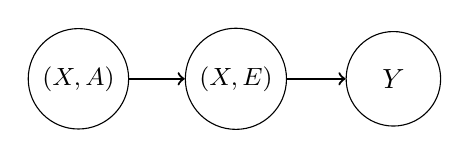
\begin{tikzpicture}

\node[circle,draw, minimum size=1.2cm] (R0) at (0,0) {\begin{small}$(X, A)$\end{small}
};
\node[circle,draw, minimum size=1.2cm] (R1) at (2,0) {\begin{small}$(X, E)$\end{small}};
\node[circle,draw, minimum size=1.2cm] (Y) at (4,0) {$Y$};

\path[->, thick] (R0) edge (R1);
\path[->, thick] (R1) edge (Y);

\end{tikzpicture}
\caption{Bayesian network corresponding to Assumption \ref{assum:indep-mips}.}
\label{fig:embedding_mips}
\vspace{-0.2cm}
%
\end{figure}


\myparagraph{Intuition}
The context-embedding pair $(X, E)$ can be seen as a representation of the context-action pair $(X, A)$ which contains less `redundant information' regarding the outcome $Y$. Intuitively, the MIPS estimator, which only considers the shift in the distribution of $(X, E)$ is therefore more efficient than the IPW estimator (which considers the shift in the distribution of $(X, A)$ instead). 
%

\myparagraph{MR achieves lower variance than MIPS}
Given the intuition above, we should achieve greater variance reduction as the amount of redundant information in the representation $(X, E)$ decreases. We formalise this in Appendix \ref{app:gmips} and show that the variance of MIPS estimator decreases as the representation gets closer to $Y$ in terms of information content. As a result, we achieve the greatest variance reduction by considering the marginal shift in the outcome $Y$ itself (as in MR) rather than the shift in the representation $(X, E)$ (as in MIPS). The following result formalizes this finding. 
%
%
\begin{theorem}\label{prop:mips_main_text}
    When the weights $w(y)$, $\frac{\ptar(e, x)}{\pbeh(e, x)}$ and $\rho(a, x)$ are known exactly, then under Assumption \ref{assum:indep-mips}, 
    \begin{align*}
        \Ebeh[\thetamr] = \Ebeh[\hat{\theta}_{\textup{MIPS}}] = \Etar[Y], \quad \textup{and} \quad \Vbeh[\thetamr] \leq \Vbeh[\hat{\theta}_{\textup{MIPS}}] \leq \Vbeh[\thetaipw].
    \end{align*}
    %
    %
    %
\end{theorem}
%
This analysis provides a link between the MR and MIPS estimators in the framework of contextual bandits, and shows that the MR estimator achieves lower variance than MIPS estimator while not requiring any additional assumptions (e.g.\ Assumption \ref{assum:indep-mips} as in MIPS). We also verify this empirically in Section \ref{sec:exp-synth} by reproducing the experimental setup in \cite{saito2022off} along with the MR baseline.
%

%

%

%

\subsubsection{Weight estimation error}\label{subsec:weight-estimation-error}
%
%
%
Our analysis so far assumes prior knowledge of the behavior policy $\beh$ and the marginal ratios $w(y)$. However, in practice, both quantities are often unknown and must be estimated from data. To this end, we assume access to an additional training dataset $\Dtr = \{(x^\tr_i, a^\tr_i, y^\tr_i)\}_{i=1}^m$ (for weight estimation), in addition to the evaluation dataset $\D = \{(x_i, a_i, y_i)\}_{i=1}^n$ (for computing the OPE estimate). 
%
%
The estimation of $\hat{w}(y)$ involves a two-step process that exclusively utilizes data from $\Dtr$:
%
%
\begin{enumerate}[label=(\roman*)]
    \item First, we estimate the policy ratio $\hat{\rho}(a, x) \approx \frac{\tar(a | x)}{\beh(a | x)}$. This can be achieved by estimating the behaviour policy $\hatbeh$, and defining $\hat{\rho}(a, x)\coloneqq \frac{\tar(a\mid x)}{\hatbeh(a\mid x)}$. Alternatively, $\hat{\rho}(a, x)$ can also be estimated directly by using density ratio estimation techniques as in \cite{sondhi2020balanced}.
    \item Secondly, we estimate the weights $\hat{w}(y)$ using Eq. \eqref{eq:weights-obj-main} with $\hat{\rho}$ instead of $\rho$.
\end{enumerate}

    %
    %
    %
    %
 
%
%
%

In practice, one may consider splitting $\Dtr$ for each estimation step outlined above. Moreover,
each approximation step may introduce bias and therefore, the MR estimator may have two sources of bias.
%
%
%
%
While classical OPE methods like IPW and DR also suffer from bias because of $\hat{\rho}$ estimation, the estimation of $\hat{w}(y)$ is specific to MR. However, we show below
that given any policy ratio estimate $\hat{\rho}$, if $\hat{w}(y)$ approximates $\Ebeh[\hat{\rho}(A, X)\mid Y=y]$ `well enough' (i.e., the estimation step (ii) shown above is `accurate enough'), 
then MR achieves a lower variance than IPW and incurs little extra bias.

\begin{proposition}\label{prop:bias-and-var-main}
Suppose that the IPW and MR estimators are defined as,
\[
\approxipw \coloneqq \frac{1}{n}\sum_{i=1}^n\hat{\rho}(a_i, x_i)\, y_i, \quad \textup{and }\quad \approxmr \coloneqq \frac{1}{n}\sum_{i=1}^n\hat{w}(y_i)\, y_i,
\]
and define the approximation error as $\epsilon \coloneqq \hat{w}(Y) - \tilde{w}(Y)$, where $\tilde{w}(Y) \coloneqq \Ebeh[\hat{\rho}(A, X)\mid Y]$. Then we have that, $\textup{Bias}(\approxmr) - \textup{Bias}(\approxipw) = \Ebeh[\epsilon\,Y]$. Moreover,
%
%
%
%
%
%
%
\begin{small}
\begin{align}
    \Vbeh[\approxipw] - \Vbeh[\approxmr]
    %
    &= \frac{1}{n}(\underbrace{\Ebeh[\Vbeh[\hat{\rho}(A, X)\,Y\mid Y]]}_{\geq 0} - \Vbeh[\epsilon\,Y] - 2\,\textup{Cov}(\tilde{w}(Y)\,Y, \epsilon\,Y)). \label{eq:var-difference-approximate-weights}
\end{align}
\end{small}
%
%
%
%
%
\end{proposition}
%
\myparagraph{Intuition} The $\epsilon$ term defined in Proposition \ref{prop:bias-and-var-main} denotes the error of the second approximation step outlined above. 
As a direct consequence of this result, we show in Appendix \ref{sec:wide_nns_weight_estimation} that as the error $\epsilon$ becomes small (specifically as $\Ebeh[\epsilon^2]\rightarrow 0$), the difference between biases of MR and IPW estimator becomes negligible.
%
Likewise, the terms $\Vbeh[\epsilon\,Y]$ and $\textup{Cov}(\tilde{w}(Y)\,Y, \epsilon\,Y)$ in Eq. \eqref{eq:var-difference-approximate-weights} will also be small and as a result the variance of MR will be lower than that of IPW (as the first term is positive). 

In fact, using recent results regarding the generalisation error of neural networks \citep{lai2023generalization}, we show that when using 2-layer wide neural networks to approximate the weights $\hat{w}(y)$, the estimation error $\epsilon$ declines with increasing training data size $m$. Specifically, under certain regularity assumptions we obtain $\Ebeh[\epsilon^2] = O(m^{-2/3})$. Using this we show that as the training data size $m$ increases, the biases of MR and IPW estimators become roughly equal with a high probability, and
\[
\Vbeh[\approxipw] - \Vbeh[\approxmr] = \frac{1}{n}\,\Ebeh[\Vbeh[\hat{\rho}(A, X)\,Y\mid Y]] + O(m^{-1/3}).
\]
Therefore the variance of MR estimator falls below that of IPW for large enough $m$. The empirical results shown in Appendix \ref{subsec:mips-empirical} are consistent with this result. Due to space constraints, the main technical result has been included in Appendix \ref{sec:wide_nns_weight_estimation}.

%
%

%
%
%

%
%
%
%
%
%
%
%
%
%
%
%
%
%
%
%
%
%
%
%
%
%
%
%

%
%
 
%
%
%
%
%

\subsection{Application to causal inference}\label{subsec:application-to-causal-inference}
 Beyond contextual bandits, the variance reduction properties of the MR estimator make it highly useful in a wide variety of other applications. Here, we show one such application in the field of causal inference, where MR can be used for the estimation of average treatment effect (ATE) \citep{pearl2009causality} and leads to some desirable properties in comparison to the conventional ATE estimation approaches. Specifically, we illustrate that the MR estimator for ATE utilizes the evaluation data $\D$ more efficiently and achieves lower variance than state-of-the-art ATE estimators and consequently provides more accurate ATE estimates.
%
%
%
%
To be concrete, the goal in this setting is to estimate ATE, defined as follows:
%
\[
\ate \coloneqq \E[Y(1)-Y(0)].
\]
Here $Y(a)$ corresponds to the outcome under a deterministic policy $\pi_a(a'\mid x) \coloneqq \ind(a'=a)$. Hence any OPE estimator can be used to estimate $\E[Y(a)]$ (and therefore ATE) by considering target policy $\tar = \pi_a$.
%
%
%
An important distinction between MR and existing approaches (like IPW or DR) is that, when estimating $\E[Y(a)]$, the existing approaches only use datapoints in $\D$ with $A=a$. To see why this is the case, we note that the policy ratios $\frac{\tar(A|X)}{\beh(A|X)} = \frac{\ind(A=a)}{\beh(A|X)}$ are zero when $A\neq a$. In contrast, the MR weights $\frac{\ptar(Y)}{\pbeh(Y)}$ are not necessarily zero for datapoints with $A\neq a$, and therefore the MR estimator uses all evaluation datapoints when estimating $\E[Y(a)]$. 

As such we show that MR applied to ATE estimation leads to a smaller variance than the existing approaches. Moreover, because MR is able to use all datapoints when estimating $\E[Y(a)]$, MR will generally be more accurate than the existing methods especially in the setting where the data is imbalanced, i.e., the number of datapoints with $A=a$ is small for a specific action $a$.
In Appendix \ref{app:causal-inference}, we formalise this variance reduction of the MR ATE estimator compared to IPW and DR estimators, by deriving analogous results to Propositions \ref{prop:var_mr} and \ref{prop:var_dr}. In addition, we also show empirically in Section \ref{subsec:causal-experiments} that the MR ATE estimator outperforms the most commonly used ATE estimators.
\begin{comment}

\begin{proposition}\label{prop:bias-and-var}
Let 
\[
\thetaipw = \frac{1}{n}\hat{\rho}(a_i, x_i)\, y_i,
\]
where $\hat{\rho}(a, x)\coloneqq \tar(a\mid x)/\hatbeh(a\mid x)$. Additionally, let
\[
\thetamr = \frac{1}{n}\hat{w}(y_i)\, y_i,
\]
where $\hat{w}(y)$ satisfies Eq. $\eqref{eq:estimated-marginal-ratio}$. Then, 
\begin{align*}
    \textup{Bias}(\thetamr) &= \textup{Bias}(\thetaipw) \qquad \textup{and,} \\
    n (\Vbeh[\thetaipw] - \Vbeh[\thetamr]) 
    &= \E_{Y\sim \pbeh(Y)} \left[ \Vbeh\left[ \hat{\rho}(A, X) \mid Y \right]\, Y^2 \right].
\end{align*}
\end{proposition}
More generally, if $\hat{w}$ is a `noisy' estimate of the conditional expectation $\Ebeh[\hat{\rho}(A, X)\mid Y]$, we can obtain similar results regarding the bias and variance of the MR estimators under certain assumptions. 
\end{comment}


%

%

%



\begin{comment}
    

Specifically, the traditional IPW estimator applied to ATE estimation yields:
\[
\ateipw = \frac{1}{n} \sum_{i=1}^n \rho_{\ate}(a_i, x_i) \times y_i, \qquad \textup{where, } \qquad \rho_{\ate}(a, x) \coloneqq \frac{\mathbbm{1}(a=1) - \mathbbm{1}(a=0)}{\beh (a|x)}.
\]

Simlarly, the MR estimator can be written as
$$
\atemr = \frac{1}{n}\sum_{i=1}^n w_{\ate}(y_i)\times y_i, \qquad \textup{where, } \qquad w_{\ate}(y) = \frac{p_{\pi^{(1)}}(y) - p_{\pi^{(0)}}(y)}{\pbeh(y)},
$$ 
and $\pi^{(a)}(a'\mid x) \coloneqq \mathbbm{1}(a'=a)$ for $a\in \{0,1\}$, and $w_{\ate}(y)$ can be estimated using regression similar to Eq. \eqref{eq:weights-obj-main}.
\end{comment}
%
%
%
%

%
%
%
%
%
%
%
%
%
%
%
%
%
%
%
%
%
%
%

\section{Related Works}
\label{sec:related_works}


\noindent\textbf{Diffusion-based Video Generation. }
The advancement of diffusion models \cite{rombach2022high, ramesh2022hierarchical, zheng2022entropy} has led to significant progress in video generation. Due to the scarcity of high-quality video-text datasets \cite{Blattmann2023, Blattmann2023a}, researchers have adapted existing text-to-image (T2I) models to facilitate text-to-video (T2V) generation. Notable examples include AnimateDiff \cite{Guo2023}, Align your Latents \cite{Blattmann2023a}, PYoCo \cite{ge2023preserve}, and Emu Video \cite{girdhar2023emu}. Further advancements, such as LVDM \cite{he2022latent}, VideoCrafter \cite{chen2023videocrafter1, chen2024videocrafter2}, ModelScope \cite{wang2023modelscope}, LAVIE \cite{wang2023lavie}, and VideoFactory \cite{wang2024videofactory}, have refined these approaches by fine-tuning both spatial and temporal blocks, leveraging T2I models for initialization to improve video quality.
Recently, Sora \cite{brooks2024video} and CogVideoX \cite{yang2024cogvideox} enhance video generation by introducing Transformer-based diffusion backbones \cite{Peebles2023, Ma2024, Yu2024} and utilizing 3D-VAE, unlocking the potential for realistic world simulators. Additionally, SVD \cite{Blattmann2023}, SEINE \cite{chen2023seine}, PixelDance \cite{zeng2024make} and PIA \cite{zhang2024pia} have made significant strides in image-to-video generation, achieving notable improvements in quality and flexibility.
Further, I2VGen-XL \cite{zhang2023i2vgen}, DynamicCrafter \cite{Xing2023}, and Moonshot \cite{zhang2024moonshot} incorporate additional cross-attention layers to strengthen conditional signals during generation.



\noindent\textbf{Controllable Generation.}
Controllable generation has become a central focus in both image \citep{Zhang2023,jiang2024survey, Mou2024, Zheng2023, peng2024controlnext, ye2023ip, wu2024spherediffusion, song2024moma, wu2024ifadapter} and video \citep{gong2024atomovideo, zhang2024moonshot, guo2025sparsectrl, jiang2024videobooth} generation, enabling users to direct the output through various types of control. A wide range of controllable inputs has been explored, including text descriptions, pose \citep{ma2024follow,wang2023disco,hu2024animate,xu2024magicanimate}, audio \citep{tang2023anytoany,tian2024emo,he2024co}, identity representations \citep{chefer2024still,wang2024customvideo,wu2024customcrafter}, trajectory \citep{yin2023dragnuwa,chen2024motion,li2024generative,wu2024motionbooth, namekata2024sg}.


\noindent\textbf{Text-based Camera Control.}
Text-based camera control methods use natural language descriptions to guide camera motion in video generation. AnimateDiff \cite{Guo2023} and SVD \cite{Blattmann2023} fine-tune LoRAs \cite{hu2021lora} for specific camera movements based on text input. 
Image conductor\cite{li2024image} proposed to separate different camera and object motions through camera LoRA weight and object LoRA weight to achieve more precise motion control.
In contrast, MotionMaster \cite{hu2024motionmaster} and Peekaboo \cite{jain2024peekaboo} offer training-free approaches for generating coarse-grained camera motions, though with limited precision. VideoComposer \cite{wang2024videocomposer} adjusts pixel-level motion vectors to provide finer control, but challenges remain in achieving precise camera control.

\noindent\textbf{Trajectory-based Camera Control.}
MotionCtrl \cite{Wang2024Motionctrl}, CameraCtrl \cite{He2024Cameractrl}, and Direct-a-Video \cite{yang2024direct} use camera pose as input to enhance control, while CVD \cite{kuang2024collaborative} extends CameraCtrl for multi-view generation, though still limited by motion complexity. To improve geometric consistency, Pose-guided diffusion \cite{tseng2023consistent}, CamCo \cite{Xu2024}, and CamI2V \cite{zheng2024cami2v} apply epipolar constraints for consistent viewpoints. VD3D \cite{bahmani2024vd3d} introduces a ControlNet\cite{Zhang2023}-like conditioning mechanism with spatiotemporal camera embeddings, enabling more precise control.
CamTrol \cite{hou2024training} offers a training-free approach that renders static point clouds into multi-view frames for video generation. Cavia \cite{xu2024cavia} introduces view-integrated attention mechanisms to improve viewpoint and temporal consistency, while I2VControl-Camera \cite{feng2024i2vcontrol} refines camera movement by employing point trajectories in the camera coordinate system. Despite these advancements, challenges in maintaining camera control and scene-scale consistency remain, which our method seeks to address. It is noted that 4Dim~\cite{watson2024controlling} introduces absolute scale but in  4D novel view synthesis (NVS) of scenes.




\section{Empirical evaluation}
In this section, we provide empirical evidence to support our theoretical results by investigating the performance of our MR estimator against the current state-of-the-art OPE methods. The code to reproduce our experiments has been made available at: \href{https://github.com/faaizT/MR-OPE}{\textcolor{blue}{github.com/faaizT/MR-OPE}}.
%
%
%
%
%
%

\subsection{Experiments on synthetic data}\label{sec:exp-synth}
For our synthetic data experiment, we reproduce the experimental setup for the synthetic data experiment in \cite{saito2022off} by reusing their code with minor modifications.
%
Specifically, $\Xspace \subseteq \mathbb{R}^d$, for various values of $d$ as described below. Likewise, the action space $\Aspace = \{0, \dots, n_a-1\}$, with $n_a$ taking a range of different values. Additional details regarding the reward function, behaviour policy $\beh$, and the estimation of weights $\hat{w}(y)$ have been included in Appendix \ref{subsec:mips-empirical} for completeness. 

%
%


\myparagraph{Target policies} 
To investigate the effect of increasing policy shift, we define a class of policies,
\[
%
\pi^{\alpha^\ast}(a | x) = \alpha^\ast\,\ind(a = \arg\max_{a'\in \Aspace} q(x, a')) + \frac{1-\alpha^\ast}{|\Aspace|} \quad \textup{where} \quad q(x, a) \coloneqq \E[Y\mid X=x, A=a],
%
\]
where $\alpha^\ast \in [0, 1]$ allows us to control the shift between $\beh$ and $\tar$. In particular, as we show later, the shift between $\beh$ and $\tar$ increases as $\alpha^\ast \rightarrow 1$. Using the ground truth behaviour policy $\beh$, we generate a dataset which is split into training and evaluation datasets of sizes $m$ and $n$ respectively. 


%
%
%
%
%
%
%
%
%
%

%
%
%
%
%

%
%
%
%
%
%
%


\myparagraph{Baselines} 
We compare our estimator with DM, IPW, DR and MIPS estimators. Our setup includes action embeddings $E$ satisfying Assumption \ref{assum:indep-mips}, and so MIPS is unbiased.
%
%
Additional baselines have been considered in Appendix \ref{subsec:mips-empirical}.
For MR, we split the training data to estimate $\hatbeh$ and $\hat{w}(y)$, whereas for all other baselines we use the entire training data to estimate $\hatbeh$ for a fair comparison.
%
%
%
%
\begin{figure}[t]
     \centering
     \begin{subfigure}[b]{0.5\textwidth}
         \centering
         \includegraphics[height=1.06in]{figures/mr/ope_vs_neval_nac_100_alphatar_0_8_dimc_1000_untrunc.png}
         \caption{Results with varying evaluation data size $n$.}
         \label{fig:mse-vs-neval}
     \end{subfigure}%
     \begin{subfigure}[b]{0.5\textwidth}
         \centering
         \includegraphics[height=1.06in]{figures/mr/ope_vs_alphatar_nac_100_neval_800_dimc_1000.png}
         \caption{Results with varying $\alpha^\ast$.}
         \label{fig:mse-vs-betatar}
     \end{subfigure}\\
    \caption{Results for synthetic data experiment. In \ref{fig:mse-vs-neval} we have $\alpha^\ast=0.8$ and in \ref{fig:mse-vs-betatar} we have $n = 800$.}
    \label{fig:syn_results1}
\end{figure}

%
%
%
%
%
%
%
%
%
%
%
%
%
%
%
%
%
\myparagraph{Results}
We compute the target policy value using the $n$ evaluation datapoints. Here, the MSE of the estimators is computed over 10 different sets of logged data replicated with different seeds. The results presented have context dimension $d=1000$, number of actions $n_a=100$ and training data size $m=5000$. More experiments for a variety of parameter values are included in Appendix \ref{subsec:mips-empirical}.


%
%
%
%
%
%
%
%
%
%
%
%
%
%
%
%
%
%
%
%
%
%
%
%
%
%
%
%
%

\myparagraph{Varying number of evaluation data $n$} 
In Figure \ref{fig:mse-vs-neval} we plot the results with increasing size of evaluation data $n$ increases. MR achieves the smallest MSE among all the baselines considered when $n$ is small, with the MSE of MR being at least an order of magnitude smaller than every baseline for $n\leq 500$. This shows that MR is significantly more accurate than the baselines when the size of the evaluation data is small. As $n\rightarrow \infty$, the difference between the results for MR and MIPS decreases. However, MR attains smaller variance and MSE than MIPS generally, verifying our analysis in Section \ref{subsec:mips-comparison}.
%
%
%
Moreover, Figure \ref{fig:mse-vs-neval} shows that while the variance of MR is greater than that of DM, it still achieves the lowest MSE overall, owing to the high bias of DM.

\begin{wrapfigure}{r}{0.35\textwidth}
    \centering
    \includegraphics[width=0.35\textwidth]{figures/mr/kl-divergence-w-uncertainty.png}
    %
    %
    %
\end{wrapfigure}
\myparagraph{Varying $\alpha^\ast$}
As $\alpha^\ast$ parameter of the target policy increases, so does the shift between the policies $\beh$ and $\pi^{\alpha^\ast}$ as illustrated by the figure on the right, which plots the KL-divergence $D_{\textup{KL}}(\beh\, || \, \pi^{\alpha^\ast})$ as a function of $\alpha$.
%
%
%
Figure \ref{fig:mse-vs-betatar} plots the results for increasing policy shift. 
Overall, the MSE of MR estimator is lowest among all the baselines. Moreover, while the MSE and variance of all estimators increase with increasing $\alpha^\ast$ the increase in these quantities is lower for the MR estimator than for the other baselines. Therefore, the relative performance of MR estimator improves with increasing policy shift and MR remains robust to increase in policy shift.
%
%
%

\myparagraph{Additional ablation studies}
In Appendix \ref{subsec:mips-empirical}, we investigate the effect of varying context dimensions $d$, number of actions $n_a$ and number of training data $m$. In every case, we observe that the MR estimator has a smaller MSE than all other baselines considered. In particular, MR remains robust to increasing $n_a$ whereas the MSE and variance of IPW and DR estimators degrade substantially when $n_a \geq 2000$. Likewise, MR outperforms the baselines even when the training data size $m$ is small.

%
%
%
%
%
%
%
%
%
%
%
%
%
%
%
%
%
%
%
%
%
%
%
%
%
%
%
%
%
%
%
%
%
%
%
%
%
%
%
%
%
%
%
%
%
%
%
%
%
%
%
%
%
%
%
%
\begin{sidewaystable}[!htp]
    \centering
    \caption{Mean squared error of target policy value with standard errors over 10 different seeds for different classification datasets. Here, number of evaluation data $n=1000$, and $\alpha^\ast=0.6$.}
    \label{tab:classification-dataset-results}
    \begin{footnotesize}
    \begin{scshape}
%
%
%
%
%
%
%
%
%
%
%
%

\begin{tabular}{llllllll}
\toprule
Dataset &             Digits &               Letter &          OptDigits &          PenDigits &           SatImage  &              Mnist & CIFAR-100\\
\midrule
DM        &  0.1508$\pm$0.0015 &    0.0886$\pm$0.0026 &  0.0485$\pm$0.0016 &   0.0520$\pm$0.0016 &  0.0208$\pm$0.0009  &  0.1109$\pm$0.0014 & 0.0020$\pm$0.0001 \\
DR        &    0.1334$\pm$0.0400 &    \red{35.085$\pm$17.768} &  0.0464$\pm$0.0061 &  0.2343$\pm$0.1404 &   0.0560$\pm$0.0395 &  0.2617$\pm$0.0139 & \red{3823.9$\pm$2023.2} \\
DRos      &  0.0847$\pm$0.0025 &    0.2363$\pm$0.0586 &  0.0384$\pm$0.0025 &  0.0138$\pm$0.0029 &  0.0078$\pm$0.0008 &  0.2151$\pm$0.0061 & 0.2628$\pm$0.1087 \\
IPW       &  0.1632$\pm$0.0462 &  \red{45.253$\pm$22.057} &   0.0844$\pm$0.0056 &  0.1342$\pm$0.0531 &    0.0900$\pm$0.0676 & 0.3359$\pm$0.0118 & \red{4116.9$\pm$2097.9}\\
SwitchDR  &  0.0982$\pm$0.0032 &    0.2387$\pm$0.0507 &  0.0557$\pm$0.0047 &   0.0342$\pm$0.0090 &  0.0136$\pm$0.0012  &   0.2750$\pm$0.0102 & 1.1644$\pm$0.8227 \\
MR (Ours) &  \textbf{0.0034$\pm$0.0001} &    \textbf{0.0018$\pm$0.0004} &  \textbf{0.0006$\pm$0.0002} &  \textbf{0.0008$\pm$0.0002} &  \textbf{0.0016$\pm$0.0003} &  \textbf{0.0121$\pm$0.0009} &  \textbf{0.0007$\pm$0.0002}\\
\bottomrule
\end{tabular}

%
%
%
%
%
%
%
%
%
%
%
%
\end{scshape}
\end{footnotesize}
\end{sidewaystable}
\subsection{Experiments on classification datasets}
Following previous works on OPE in contextual bandits \citep{dudik2014doubly, kallus2021optimal, mehrdad2018more,wang2017optimal}, we transform classification datasets into contextual bandit feedback data in this experiment.
We consider five UCI classification datasets \citep{dua2019uci} as well as Mnist \citep{deng2012mnist} and CIFAR-100 \citep{krizhevsky2009learning} datasets, each of which comprises $\{(x_i, a^\gt_i)\}_{i}$, where $x_i\in \Xspace$ are feature vectors and $a^\gt_i\in \Aspace$ are the ground-truth labels.
%
%
In the contextual bandits setup, the feature vectors $x_i$ are considered to be the contexts, whereas the actions correspond to the possible class of labels. For the context vector $x_i$ and the action $a_i$, the reward $y_i$ is defined as $y_i \coloneqq \ind(a_i = a^\gt_i)$, i.e., the reward is 1 when the action is the same as the ground truth label and 0 otherwise. Here, the baselines considered include the DM, IPW and DR estimators as well as Switch-DR \citep{wang2017optimal} and DR with Optimistic Shrinkage (DRos) \citep{su2020doubly}. We do not consider a MIPS baseline here as there is no natural embedding $E$ of $A$. Additional details are provided in Appendix \ref{subsec:additional-experiments-classification}. 
%
%
%

In Table \ref{tab:classification-dataset-results}, we present the results with number of evaluation data $n=1000$ and number of training data $m=500$. 
The table shows that across all datasets, MR achieves the lowest MSE among all methods. \flag{Moreover, for the Letter and CIFAR-100 datasets the IPW and DR yield large bias and variance arising from poor policy estimates $\hatbeh$. Despite this, the MR estimator which utilizes the \emph{same} $\hatbeh$ for the estimation of $\hat{w}(y)$ leads to much more accurate results.} We also verify that MR outperforms the baselines for increasing policy shift and evaluation data $n$ in Appendix \ref{subsec:additional-experiments-classification}.
%


%

%

%
%
%
%
%

\subsection{Application to ATE estimation}\label{subsec:causal-experiments}
%
In this experiment, we investigate the empirical performance of the MR estimator for ATE estimation. 

\myparagraph{Twins dataset}
We use the Twins dataset studied in \cite{louizos2017causal}, which comprises data from twin births in the USA between 1989-1991. The treatment $a=1$ corresponds to being born the heavier twin and the outcome $Y$ corresponds to the mortality of each of the twins in their first year of life. Specifically, $Y(1)$ corresponds to the mortality of the heavier twin (and likewise for $Y(0)$). To simulate the observational study, we follow a similar strategy as in \cite{louizos2017causal} to selectively hide one of the two twins as explained in Appendix \ref{app:ate-empirical}. We obtain a total of 11,984 datapoints, of which 5000 datapoints are used to train the behaviour policy $\hatbeh$ and outcome model $\hat{q}(x, a)$.

%
%

%
\begin{table}[t]
%
    \centering
    \caption{Mean absolute ATE estimation error $\epsilon_\ate$ with standard errors over 10 different seeds, for increasing number of evaluation data $n$.}
    \label{tab:ate_errors-main}
    \begin{small}
    \begin{tabular}{lllll}
\toprule
$n$ &             50   &             200  &             1600 &             3200 \\
\midrule
DM       &  0.092$\pm$0.003 &  0.092$\pm$0.003 &  0.092$\pm$0.004 &  0.092$\pm$0.004 \\
DR       &  0.101$\pm$0.024 &  \textbf{0.065$\pm$0.009} &  0.071$\pm$0.005 &  0.069$\pm$0.004 \\
\textsc{DRos}     &    0.100$\pm$0.017 &  0.089$\pm$0.006 &   0.093$\pm$0.004 &  0.087$\pm$0.004 \\
IPW      &  0.092$\pm$0.024 &  0.088$\pm$0.014 &  0.067$\pm$0.007 &  0.067$\pm$0.007 \\
\textsc{SwitchDR} &  0.101$\pm$0.024 &  \textbf{0.065$\pm$0.009} &  0.071$\pm$0.005 &  0.069$\pm$0.004 \\
MR (Ours)      &  \textbf{0.062$\pm$0.007} &  \textbf{0.065$\pm$0.007} &  \textbf{0.061$\pm$0.005} &  \textbf{0.061$\pm$0.006} \\
\bottomrule
\end{tabular}
\end{small}
%
\end{table}
%
Here, we consider the same baselines as the classification data experiments in previous section.
For our evaluation, we consider the absolute error in ATE estimation, $\epsilon_\ate$, defined as:
$
\epsilon_\ate \coloneqq | \hat{\theta}^{(n)}_\ate - \theta_\ate |.
$
Here, $\hat{\theta}^{(n)}_\ate$ denotes the value of the ATE estimated using $n$ evaluation datapoints.
%
We compute the ATE value using the $n$ evaluation datapoints, over 10 different sets of observational data (using different seeds). Table \ref{tab:ate_errors-main} shows that MR achieves the lowest estimation error $\epsilon_\ate$ for all values of $n$ considered here. While the performance of other baselines improves with increasing $n$, MR outperforms them all. 
%


%
%
%
%
%
%
%
%
%
%
%
%
%
%
%
%
%
%
%


%
%
%

%
%

\section{Discussion of Assumptions}\label{sec:discussion}
In this paper, we have made several assumptions for the sake of clarity and simplicity. In this section, we discuss the rationale behind these assumptions, the extent to which these assumptions hold in practice, and the consequences for our protocol when these assumptions hold.

\subsection{Assumptions on the Demand}

There are two simplifying assumptions we make about the demand. First, we assume the demand at any time is relatively small compared to the channel capacities. Second, we take the demand to be constant over time. We elaborate upon both these points below.

\paragraph{Small demands} The assumption that demands are small relative to channel capacities is made precise in \eqref{eq:large_capacity_assumption}. This assumption simplifies two major aspects of our protocol. First, it largely removes congestion from consideration. In \eqref{eq:primal_problem}, there is no constraint ensuring that total flow in both directions stays below capacity--this is always met. Consequently, there is no Lagrange multiplier for congestion and no congestion pricing; only imbalance penalties apply. In contrast, protocols in \cite{sivaraman2020high, varma2021throughput, wang2024fence} include congestion fees due to explicit congestion constraints. Second, the bound \eqref{eq:large_capacity_assumption} ensures that as long as channels remain balanced, the network can always meet demand, no matter how the demand is routed. Since channels can rebalance when necessary, they never drop transactions. This allows prices and flows to adjust as per the equations in \eqref{eq:algorithm}, which makes it easier to prove the protocol's convergence guarantees. This also preserves the key property that a channel's price remains proportional to net money flow through it.

In practice, payment channel networks are used most often for micro-payments, for which on-chain transactions are prohibitively expensive; large transactions typically take place directly on the blockchain. For example, according to \cite{river2023lightning}, the average channel capacity is roughly $0.1$ BTC ($5,000$ BTC distributed over $50,000$ channels), while the average transaction amount is less than $0.0004$ BTC ($44.7k$ satoshis). Thus, the small demand assumption is not too unrealistic. Additionally, the occasional large transaction can be treated as a sequence of smaller transactions by breaking it into packets and executing each packet serially (as done by \cite{sivaraman2020high}).
Lastly, a good path discovery process that favors large capacity channels over small capacity ones can help ensure that the bound in \eqref{eq:large_capacity_assumption} holds.

\paragraph{Constant demands} 
In this work, we assume that any transacting pair of nodes have a steady transaction demand between them (see Section \ref{sec:transaction_requests}). Making this assumption is necessary to obtain the kind of guarantees that we have presented in this paper. Unless the demand is steady, it is unreasonable to expect that the flows converge to a steady value. Weaker assumptions on the demand lead to weaker guarantees. For example, with the more general setting of stochastic, but i.i.d. demand between any two nodes, \cite{varma2021throughput} shows that the channel queue lengths are bounded in expectation. If the demand can be arbitrary, then it is very hard to get any meaningful performance guarantees; \cite{wang2024fence} shows that even for a single bidirectional channel, the competitive ratio is infinite. Indeed, because a PCN is a decentralized system and decisions must be made based on local information alone, it is difficult for the network to find the optimal detailed balance flow at every time step with a time-varying demand.  With a steady demand, the network can discover the optimal flows in a reasonably short time, as our work shows.

We view the constant demand assumption as an approximation for a more general demand process that could be piece-wise constant, stochastic, or both (see simulations in Figure \ref{fig:five_nodes_variable_demand}).
We believe it should be possible to merge ideas from our work and \cite{varma2021throughput} to provide guarantees in a setting with random demands with arbitrary means. We leave this for future work. In addition, our work suggests that a reasonable method of handling stochastic demands is to queue the transaction requests \textit{at the source node} itself. This queuing action should be viewed in conjunction with flow-control. Indeed, a temporarily high unidirectional demand would raise prices for the sender, incentivizing the sender to stop sending the transactions. If the sender queues the transactions, they can send them later when prices drop. This form of queuing does not require any overhaul of the basic PCN infrastructure and is therefore simpler to implement than per-channel queues as suggested by \cite{sivaraman2020high} and \cite{varma2021throughput}.

\subsection{The Incentive of Channels}
The actions of the channels as prescribed by the DEBT control protocol can be summarized as follows. Channels adjust their prices in proportion to the net flow through them. They rebalance themselves whenever necessary and execute any transaction request that has been made of them. We discuss both these aspects below.

\paragraph{On Prices}
In this work, the exclusive role of channel prices is to ensure that the flows through each channel remains balanced. In practice, it would be important to include other components in a channel's price/fee as well: a congestion price  and an incentive price. The congestion price, as suggested by \cite{varma2021throughput}, would depend on the total flow of transactions through the channel, and would incentivize nodes to balance the load over different paths. The incentive price, which is commonly used in practice \cite{river2023lightning}, is necessary to provide channels with an incentive to serve as an intermediary for different channels. In practice, we expect both these components to be smaller than the imbalance price. Consequently, we expect the behavior of our protocol to be similar to our theoretical results even with these additional prices.

A key aspect of our protocol is that channel fees are allowed to be negative. Although the original Lightning network whitepaper \cite{poon2016bitcoin} suggests that negative channel prices may be a good solution to promote rebalancing, the idea of negative prices in not very popular in the literature. To our knowledge, the only prior work with this feature is \cite{varma2021throughput}. Indeed, in papers such as \cite{van2021merchant} and \cite{wang2024fence}, the price function is explicitly modified such that the channel price is never negative. The results of our paper show the benefits of negative prices. For one, in steady state, equal flows in both directions ensure that a channel doesn't loose any money (the other price components mentioned above ensure that the channel will only gain money). More importantly, negative prices are important to ensure that the protocol selectively stifles acyclic flows while allowing circulations to flow. Indeed, in the example of Section \ref{sec:flow_control_example}, the flows between nodes $A$ and $C$ are left on only because the large positive price over one channel is canceled by the corresponding negative price over the other channel, leading to a net zero price.

Lastly, observe that in the DEBT control protocol, the price charged by a channel does not depend on its capacity. This is a natural consequence of the price being the Lagrange multiplier for the net-zero flow constraint, which also does not depend on the channel capacity. In contrast, in many other works, the imbalance price is normalized by the channel capacity \cite{ren2018optimal, lin2020funds, wang2024fence}; this is shown to work well in practice. The rationale for such a price structure is explained well in \cite{wang2024fence}, where this fee is derived with the aim of always maintaining some balance (liquidity) at each end of every channel. This is a reasonable aim if a channel is to never rebalance itself; the experiments of the aforementioned papers are conducted in such a regime. In this work, however, we allow the channels to rebalance themselves a few times in order to settle on a detailed balance flow. This is because our focus is on the long-term steady state performance of the protocol. This difference in perspective also shows up in how the price depends on the channel imbalance. \cite{lin2020funds} and \cite{wang2024fence} advocate for strictly convex prices whereas this work and \cite{varma2021throughput} propose linear prices.

\paragraph{On Rebalancing} 
Recall that the DEBT control protocol ensures that the flows in the network converge to a detailed balance flow, which can be sustained perpetually without any rebalancing. However, during the transient phase (before convergence), channels may have to perform on-chain rebalancing a few times. Since rebalancing is an expensive operation, it is worthwhile discussing methods by which channels can reduce the extent of rebalancing. One option for the channels to reduce the extent of rebalancing is to increase their capacity; however, this comes at the cost of locking in more capital. Each channel can decide for itself the optimum amount of capital to lock in. Another option, which we discuss in Section \ref{sec:five_node}, is for channels to increase the rate $\gamma$ at which they adjust prices. 

Ultimately, whether or not it is beneficial for a channel to rebalance depends on the time-horizon under consideration. Our protocol is based on the assumption that the demand remains steady for a long period of time. If this is indeed the case, it would be worthwhile for a channel to rebalance itself as it can make up this cost through the incentive fees gained from the flow of transactions through it in steady state. If a channel chooses not to rebalance itself, however, there is a risk of being trapped in a deadlock, which is suboptimal for not only the nodes but also the channel.

\section{Conclusion}
This work presents DEBT control: a protocol for payment channel networks that uses source routing and flow control based on channel prices. The protocol is derived by posing a network utility maximization problem and analyzing its dual minimization. It is shown that under steady demands, the protocol guides the network to an optimal, sustainable point. Simulations show its robustness to demand variations. The work demonstrates that simple protocols with strong theoretical guarantees are possible for PCNs and we hope it inspires further theoretical research in this direction.